% -----------------------------------------------------------------------------
%                                     HEADER                                    
% -----------------------------------------------------------------------------
\documentclass[a4paper, 11pt]{article}
\usepackage{jheppub}
\usepackage[T1]{fontenc}
\usepackage{colortbl}
\definecolor{orange}{rgb}{1,0.5,0}
% -----------------------------------------------------------------------------
%                                   COVER PAGE                                  
% -----------------------------------------------------------------------------
\title{{
\includegraphics[scale=.4]{logo.png}}\ The LaTeX report}

\author{Generated by local1 on 30 September 2014, 15:59:57}

\abstract{
  This report has been generated automatically
  by {\sc MadAnalysis} 5.\\$~$\\ 
  Please cite:\\ 
  \begin{quote}
    \textbf{E.~Conte, B.~Fuks and G.~Serret},\\ 
    \textit{MadAnalysis 5, A User-Friendly
    Framework for Collider Phenomenology},\\ 
    Comput. Phys. Commun. {\bf 184} (2013) 222-256,\\
    arXiv:1206.1599 [hep-ph].\\ 
  \end{quote}
  To contact us:\\ 
  \begin{quote}
    \textbf{http://madanalysis.irmp.ucl.ac.be}\\
    \textbf{ma5team@iphc.cnrs.fr}\\
  \end{quote}
}

% -----------------------------------------------------------------------------
%                                 BEGIN DOCUMENT                                
% -----------------------------------------------------------------------------
\begin{document}
\maketitle
\flushbottom

% -----------------------------------------------------------------------------
%                                 SECTION Setup                                 
% -----------------------------------------------------------------------------
\newpage
\section{ Setup}

\subsection{ Command history}

\texttt{ ma5>import ../\-../\-../\-madgraph/\-e+e-2yy/\-Events/\-run\_11/\-unweighted\_events.lhe.gz\\
}
\texttt{ }\texttt{ }\texttt{ ma5>import ../\-../\-../\-madgraph/\-e+e-2yy/\-Events/\-run\_11/\-unweighted\_events.lhe\\
}
\texttt{ }\texttt{ }\texttt{ ma5>plot MET\\
}
\texttt{ }\texttt{ }\texttt{ ma5>plot PT(a) 20 0 100\\
}
\texttt{ }\texttt{ }\texttt{ ma5>generate pdflatex test.pdf\\
}
\texttt{ }\texttt{ }\texttt{ ma5>generate\_pdflatex test.pdf\\
}
\texttt{ }\texttt{ }\texttt{ ma5>submit test\\
}
\texttt{ }\texttt{ }\subsection{ Configuration}

\begin{itemize}
  \item MadAnalysis version 1.1.11 (2014/\-09/\-15).
   \item Histograms given for an integrated luminosity of \textcolor{blue}{10}\textcolor{blue}{ fb}$^{\textcolor{blue}{-1}}$\textcolor{blue}{.}
\textcolor{blue}{}
\end{itemize}
% -----------------------------------------------------------------------------
%                                SECTION Datasets                               
% -----------------------------------------------------------------------------
\newpage
\section{ Datasets}

\subsection{ defaultset}

\begin{itemize}
  \item Samples stored in the directory: \textcolor{blue}{/\-media/\-sf\_darkphotons/\-madanalysis/\-madanalysis5/\-bin} .
   \item Sample consisting of: \textcolor{blue}{signal}  events.
   \item Generated events: \textcolor{blue}{100000 }  events.
   \item Normalization to the luminosity: \textcolor{blue}{1449369000000}\textcolor{blue}{ +/\-- }\textcolor{blue}{91748050 }  events.
   \item\textcolor{red}{Ratio (event weight): }\textcolor{red}{14493690 }\textcolor{red}{ - warning: please generate more events (weight larger than 1)!}
\textcolor{red}{}
\end{itemize}
\begin{table}[!h]
  \begin{center}
    \begin{tabular}{|m{51.0mm}|m{24.0mm}|m{28.0mm}|m{28.0mm}|}
      \hline
      \cellcolor{yellow}         Path to the event file& \cellcolor{yellow}         Nr. of events& \cellcolor{yellow}         Cross section (pb)& \cellcolor{yellow}         Negative wgts (\%)\\
      \hline
      \cellcolor{white}          /\-media/\-sf\_darkphotons/\-madgraph/\-e+e-2yy/\-Events/\-run\_11/\-unweighted\_events.lhe& \cellcolor{white}          100000& \cellcolor{white}          144936900 @ 0.0063\%& \cellcolor{white}          0.0\\
\hline
    \end{tabular}
  \end{center}
\end{table}

% -----------------------------------------------------------------------------
%                            SECTION Histos and cuts                            
% -----------------------------------------------------------------------------
\newpage
\section{ Histos and cuts}

\subsection{ Histogram 1}

   \textbf{   * Plot: MET}
\textbf{ }\begin{table}[!h]
  \begin{center}
    \caption{ Statistics table}
    \begin{tabular}{|m{17.0mm}|m{27.0mm}|m{23.0mm}|m{18.0mm}|m{18.0mm}|m{14.0mm}|m{14.0mm}|}
      \hline
      \cellcolor{yellow}         Dataset& \cellcolor{yellow}         Integral& \cellcolor{yellow}         Entries /\- events& \cellcolor{yellow}         Mean& \cellcolor{yellow}         RMS& \cellcolor{yellow}         \%Underflow& \cellcolor{yellow}         \%Overflow\\
      \hline
      \cellcolor{white}         defaultset& \cellcolor{white}         1.449369e+12& \cellcolor{white}         1.0& \cellcolor{white}         0.0& \cellcolor{white}         0.0& \cellcolor{green}         0.0& \cellcolor{green}         0.0\\
\hline
    \end{tabular}
  \end{center}
\end{table}

\begin{figure}[!h]
  \begin{center}
    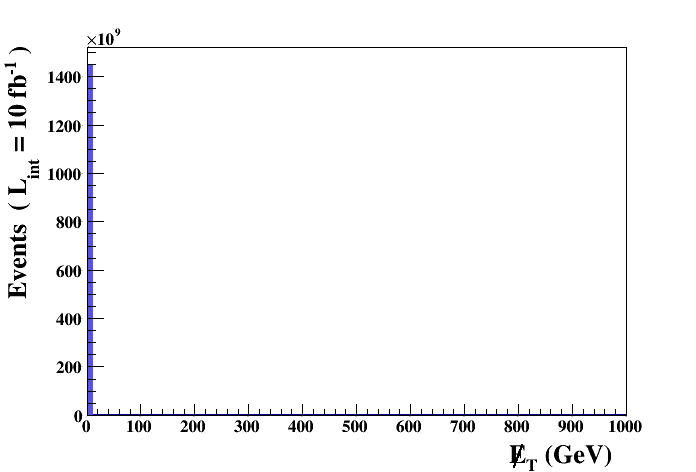
\includegraphics[scale=0.6]{selection_0.png}\\
\caption{}
  \end{center}
\end{figure}
\newpage
   \newpage
\subsection{ Histogram 2}

   \textbf{   * Plot: PT ( a ) }
\textbf{ }\begin{table}[!h]
  \begin{center}
    \caption{ Statistics table}
    \begin{tabular}{|m{17.0mm}|m{27.0mm}|m{23.0mm}|m{18.0mm}|m{18.0mm}|m{14.0mm}|m{14.0mm}|}
      \hline
      \cellcolor{yellow}         Dataset& \cellcolor{yellow}         Integral& \cellcolor{yellow}         Entries /\- events& \cellcolor{yellow}         Mean& \cellcolor{yellow}         RMS& \cellcolor{yellow}         \%Underflow& \cellcolor{yellow}         \%Overflow\\
      \hline
      \cellcolor{white}         defaultset& \cellcolor{white}         2.898738e+12& \cellcolor{white}         2.0& \cellcolor{white}         0.0146585& \cellcolor{white}         0.01015& \cellcolor{green}         0.0& \cellcolor{green}         0.0\\
\hline
    \end{tabular}
  \end{center}
\end{table}

\begin{figure}[!h]
  \begin{center}
    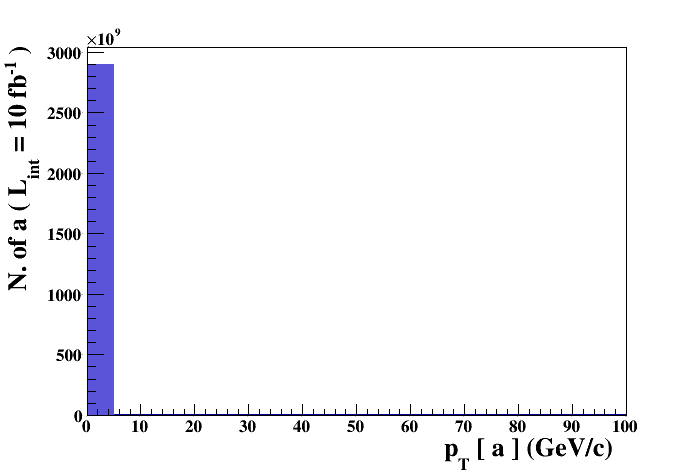
\includegraphics[scale=0.6]{selection_1.png}\\
\caption{}
  \end{center}
\end{figure}
\newpage
   \end{document}
